%% paper.tex


\documentclass[pldi]{sigplanconf-pldi16}

% standard LaTeX packages

% standard LaTeX packages
%\usepackage{changebar}

\usepackage{balance}
\usepackage{alltt}
\usepackage{amsmath}
\usepackage{balance}
\usepackage{booktabs}
\usepackage{fixltx2e}
\usepackage{graphicx}
\usepackage{boxedminipage}
\usepackage{hyperref}
\usepackage{nicefrac}
\usepackage{subfig}
\usepackage{xcolor}
\usepackage{setspace}
\usepackage{xspace}
\usepackage{multirow}
\usepackage{colortbl}
\usepackage{amsfonts} 
\usepackage{blindtext}
\usepackage{chngpage}
\usepackage{listings}
\usepackage{mathtools}
\usepackage{amssymb}
\usepackage{pifont}
%\usepackage{pgfplotstable}

\usepackage[linesnumbered, vlined, ruled]{algorithm2e}
% font selection
%\usepackage{courier}
%\usepackage[scaled]{helvet}
\usepackage{mathptmx}
\usepackage{times}

% custom packages for this paper
\usepackage{double-blind}
\usepackage{shared-affiliation}

\usepackage[numbers,sort&compress,square]{natbib}

\lstset{
  basicstyle=\tiny,
  columns=fullflexible,
  numbersep=5pt,
  numberstyle=\scriptsize,
  showstringspaces=false,
  escapeinside={/*@}{@*/},
  belowcaptionskip=1\baselineskip,
  language=C,
  showstringspaces=true,
  keywordstyle=\bfseries,
  commentstyle=\itshape,
}


%\pgfplotstableset{
%    color cells/.style={
%        col sep=comma,
%        string type,
%        postproc cell content/.code={%
%                \pgfkeysalso{@cell content=\rule{0cm}{2.4ex}\cellcolor{black!##10}\pgfmathtruncatemacro\number{##1}\ifnum\number>5\color{white}\fi##1}%
%                },
%        columns/x/.style={
%            column name={},
%            postproc cell content/.code={}
%        }
%    }
%}



\newcommand{\Code}[1]{\lstinline{#1}}
\newcommand{\Tool}{LDoctor\xspace}

\makeatletter
\def\@copyrightspace{\relax}
\makeatother

\captionsetup{format=default, font=bf}

%\newcommand{\allbugs}{110\xspace}
%\newcommand{\allbugsns}{110}
%\newcommand{\usefulp}{54\xspace}
%\newcommand{\usefulsp}{25\xspace}
%\newcommand{\newbug}{61\xspace}
%\newcommand{\newconfirm}{1\xspace}
%\newcommand{\newrepeated}{0\xspace}
%\newcommand{\mailto}[1]{\href{mailto:#1}{#1}}
\newcommand*{\Scale}[2][4]{\scalebox{#1}{$#2$}}%
\newcommand{\comment}[1]{{}}

%% taken from unknown.sty
%\DeclareCaptionType{copyrightbox}

\sloppy

\begin{document}

\title{
  Performance Diagnosis for Inefficient Loops
}

\input macros.tex

%\numberofauthors{2}
\authorinfo{Linhai Song \and Shan Lu\thanks{Shan is now with University of Chicago.}}
           {University of Wisconsin--Madison}
           {\{songlh, shanlu\}@cs.wisc.edu}
\maketitle
\begin{abstract}
\input section/abstract.tex
\end{abstract}

\section{Introduction}
\label{sec:intro}
\subsection{Motivation}

Performance bugs\footnote{We also refer performance bugs as performance problems
following previous works in this area~\cite{PerfBug,Alabama,SongOOPSLA2014}} 
are software implementation mistakes that cause unnecessary performance
degradation in software. They widely exist in deployed software due to the 
complexity of modern software
~\cite{PerfBug,perf.fse10,rily.perftest,perfantipattern,xiao13:context}. 
They annoy end users and waste energy during production runs, and 
have already caused highly publicized failures~\cite{ACA-health,colorado}.
Tools that can help
developers quickly and accurately diagnose performance problems
are sorely desired.

Performance diagnosis is different from performance testing or
bug detection: it does \textit{not} aim to expose previously unknown performance
anomalies. 
Instead, it is similar with general failure diagnosis: 
it is applied \textit{after} an unexpected software behavior (i.e., symptom)
is observed, hoping to identify the root cause of this symptom and suggest
strategies to eliminate this symptom.
In the context of performance problems, the symptom is execution 
slowness \cite{SongOOPSLA2014}; the root cause is about
which code region is inefficient and why.
An effective diagnosis tool can help developers quickly and correctly understand 
and fix already-exposed performance symptoms.

Also like general failure diagnosis, ideal performance diagnosis tools should
satisfy three criteria.
\begin{itemize}
\item Coverage. 
Real-world performance problems are caused by a wide variety of reasons.
A good diagnosis tool should handle a good portion of them.

\item Accuracy. 
Which code regions are inefficient and why they are inefficient
need to be accurately identified.

\item Performance. 
Diagnosis often requires collecting run-time information. The lower the overhead
is, the easier for the tool to deploy, especially for 
production-run usage. 
\end{itemize}

No existing tools can satisfy these
three requirements.

Profiling is the state of practice in performance diagnosis.
It is far from providing the desired \textit{accuracy}, as it is designed to
tell where computation resources are spent, 
but not where and why resources are wasted. 
In many cases, the root-cause function may not even
get ranked by the profiler \cite{SongOOPSLA2014}.

Performance bug detection tools use program analysis to identify
code regions that match specific inefficiency patterns 
\cite{Alabama,CARAMEL, Cachetor,Xu:2010:FLD:1806596.1806617,Dufour:2008:STC:1453101.1453111, Xu:2009:GFP:1542476.1542523, Xu:2010:DIC:1806596.1806616,IsilDillig.PLDI15}. 
Unfortunately, these tools are not designed and hence are unsuitable
to identify code regions that contribute to a specific slowness symptom.
They do not provide \textit{coverage} for a wide
variety of real-world problems; they are not guided by
performance failure symptoms, and hence are at disadvantage in terms of diagnosis
\textit{accuracy}; dynamic detection tools often lead to 
10X slowdowns or more \cite{Cachetor,Xu:2010:FLD:1806596.1806617,Alabama}, 
not ideal in terms of \textit{performance}.

Recently, progress has been made on statistical debugging for
performance diagnosis \cite{SongOOPSLA2014}.
This approach compares runs with and without problematic performance, and
identifies control-flow constructs, such as a branch $b$ or 
a loop $l$, that are most correlated with
the execution slowness.
Unfortunately, this approach is \textit{not} effective
for loop-related 
performance problems, which contribute to two thirds of
real-world performance problems studied in previous work 
\cite{SongOOPSLA2014,PerfBug}. It cannot
tell whether and how loop $l$ is inefficient 
and hence is limited in its diagnosis \textit{coverage} and \textit{accuracy}.

\begin{figure}
\centering
\lstset{basicstyle=\ttfamily\fontsize{8}{8}\selectfont,
     morekeywords={+},keepspaces=true}
  \mbox{\lstinputlisting[mathescape,boxpos=t]{figures/GCC27733.c}}
\caption{A real-world performance bug in GCC (the `-' and `+' demonstrate the patch; variable and 
function names are simplified for demonstration purposes)}
\label{fig:GCC27733}
\end{figure}

Figure~\ref{fig:GCC27733} shows a performance problem in GCC. 
Recursive function \texttt{mult\_alg} computes the best algorithm for 
multiplying \texttt{t}, a time-consuming computation. 
At run time, \texttt{mult\_alg} is often invoked for many times, and often
with the same parameter partly due to its recursive nature.
To avoid redundant computation across different instances of
\texttt{mult\_alg}, developers used a
hash-table
\texttt{alg\_hash} to remember which parameter \texttt{t} has been processed
in the past and what is the result. 
Unfortunately, a mistake in the type declaration of hash-table
entry \texttt{hash\_entry} makes the memoization useless for large \texttt{t}.
In many cases, a slow path is taken, when the fast path should have been taken.
This mistake does not affect software correctness, but causes a large amount
of redundant computation\footnote{This will be considered as a
loop-redundancy problem later in this paper, as we consider
recursive functions as a special case of loops.} 
and hurts GCC performance severely,
causing hundreds of times slow down for GCC test cases.

Debugging this performance problem is challenging. According to 
the discussion forum of GCC, developers identified
\texttt{mult\_alg} as the most time-consuming function
through profilers early on. However, they did not figure out 
whether \texttt{mult\_alg} is inefficient, which part of it is 
inefficient (\texttt{mult\_alg} is a large function with about 400 lines of 
code), and how it is inefficient, until several weeks later.

If a tool can tell developers not only \emph{which} loop or function is
responsible for execution slowness, but also \emph{why} and \emph{how}
it is inefficient, 
diagnosis and fixing
would be much easier. 

\iffalse
%to save space
Clearly, more research is needed to improve the state of the art of performance
diagnosis --- better diagnosis
coverage, better diagnosis accuracy, and low run-time
overhead for common performance problems,
especially loop-related performance problems.
\fi


\subsection{Contributions}
This paper presents a tool \Tool that can help effectively diagnose
inefficient loop problems, the most common type of performance problems
\cite{SongOOPSLA2014,PerfBug}, with good coverage, accuracy, and performance.
After users or developers observe a performance failure symptom, \Tool can 
automatically judge whether the symptom is caused by inefficient loops and
provide detailed root-cause information that helps understand and fix 
inefficient loops. 


\Tool tackles this challenging problem in three steps.
%}

First, figuring out a root-cause taxonomy for inefficient loops.
%Specifically, we consider \textit{resultless} and
%\textit{redundancy} as two main categories of root causes for inefficient
%loops, representing loops that spend effort without producing
%any results or producing redundant results. They are further divided into
%sub-categories based on the granularity of the resultless or redundant work. 
Our taxonomy categorizes all inefficient loops into two main categories:
\emph{resultless}, when a large amount of computation produces
no side effects, and \emph{redundancy}, when a large amount of 
computation produces already-available results.
Each main category is further divided to sub-categories.
We strive to make the taxonomy both general enough to cover
common inefficient loops, and specific enough to guide the design
of \Tool and eventually help developers understand
and fix performance problems
(Section \ref{sec:study}).
 
Second, building a tool(kit) \Tool that can automatically and accurately
identify whether and how a suspicious loop is inefficient, 
following these principles (Section \ref{sec:design}):

\begin{itemize}
\item Focused checking. 
Different from performance-bug detectors that blindly check the whole
software, \Tool focuses on loops that are
most correlated with performance symptoms. 
This focus is crucial for \Tool to achieve both high
accuracy and high coverage.

\item Taxonomy guided design. To provide good coverage, we follow
the root-cause taxonomy discussed above and design analysis routines for
every root-cause category. Given a candidate loop, \Tool
applies a series of analysis to see if it matches any type of inefficiency.
%We will also put the analysis results from different analysis routines together
%to figure out the most likely root cause category for an inefficient loop.

\item Static-dynamic hybrid analysis.
Static analysis alone cannot accurately identify 
inefficiency root causes, as some inefficiency only
happens or matters under specific workload; dynamic analysis alone will 
cause too large 
run-time overhead. Therefore, we use a hybrid approach to achieve both
performance and accuracy goals.
\end{itemize}

Third, using sampling to further lower the run-time overhead of \Tool, without
degrading diagnosis capability. Random sampling is a natural fit for performance
diagnosis due to the repetitive nature of inefficient loops (Section \ref{sec:inst}).

We evaluated \Tool on \allbugs real-world performance problems,
coming from two representative benchmark suites 
\cite{SongOOPSLA2014,Alabama}. 
Evaluation results show that \Tool can accurately identify detailed
root cause for all benchmarks and provide correct fix-strategy suggestion for
most benchmarks. All of these are achieved with low run-time overhead.

\section{Root-Cause Taxonomy}
\label{sec:study}

To guide the design of automated diagnosis tools, we need a
taxonomy for inefficient loops that satisfies three requirements:
(1) \textit{Coverage}, covering
a big portion of real-world inefficient loop problems; 
(2) \textit{Actionability}, each root-cause category being informative enough 
to help developers fix a performance problem; 
(3) \textit{Generality}, allowing automated diagnosis to be applied to many
applications.

Previous work identified a wide variety of performance root-cause 
categories. However, existing taxonomies do not satisfy all these 
requirements and hence cannot be directly used by us.
Therefore, we have designed our own taxonomy,
as presented below.
We will discuss how our taxonomy meets these three requirements
qualitatively in this section and quantitatively 
using real-world performance-bug suite in Section \ref{sec:eval_taxonomy}.


\subsection{Resultless loops}
\label{sec:study_resultless}
Resultless loops spend a lot of time in computation that does not
produce results useful after the loop (i.e., no side effects).
They can be further categorized to four sub-types 
based on which part of the loop is
(not) producing useful results.


{\textbf{0*}} loops
never produce any results in any iteration.
They are rare in mature software systems.

{\textit{How to fix?}} They should be deleted from software.
%Question: dynamic or static?

\begin{figure}
\centering
\lstset{basicstyle=\ttfamily\fontsize{8}{8}\selectfont,
     morekeywords={+},keepspaces=true,numbers=left}
  \mbox{\lstinputlisting[mathescape,boxpos=t]{figures/Mozilla347306.c}}
\caption{A resultless 0*1? bug in Mozilla}
\label{fig:Mozilla347306}
\end{figure}

{\textbf{0*1?}} loops only produce results in the last iteration, if any. 
They are often related to search: check a sequence of elements one
by one until the right one is found.
Whether these loops are efficient or not depends on the
workload. 
An example is shown in Figure \ref{fig:Mozilla347306}.
Large JavaScript files often fill the \texttt{script} list with 
tens of thousands of nodes and cause poor performance.

{\textit{How to fix?}}
They are often fixed by data-structure changes.
For example, the patch for the bug in Figure \ref{fig:Mozilla347306}
simply replaced the \texttt{script} list with a hash table.
% This improve the performance by 52.60{\bf X}.

\comment{
This loop searches through xxx for xxx.
When xx, this loop often needs to execute xx iterations, which is very
time consuming.
The developers simply change the data-structure of xx from xx to a hash
table, which eliminates this loop and improving the performance by xxx.}
%Linhai, you have to describe examples using words people can understand
%and you have to provide useful information, such as what is the purpose
% of the loop. What is the loop searching for? What is the bug-triggering
%workload; how bad the performance (throughput or latency) was; how good
%is the fixed version in terms of performance.
\comment{
\textcolor{red}{
MySQL\#27287 is caused by linear backward searching for parent node during XML string parsing. 
In each iteration of the buggy loop, one previous sibling will be skipped, 
and in the last iteration, parent node will be returned. 
The patch applies a stack-like data structure to keep all parent nodes who have unparsed children to avoid the linear backward searching.
} } 
%Linhai, I have no idea what you are talking about here for mysql27287

%TOADD: performance diagnosis is different from bug detection%
%in many cases, there is no absolutely ``bad'' cases. performance problems are
%often a trade-off between code simplicity, performance, xxx.
%treating it like bug detection will inevitably lead to false positives
%we are providing information to developers


{\textbf{[0$|$1]*}} loops may or may not produce results in each
iteration.
For some workload, the majority of iterations do not produce
results and cause performance problems perceived by users.
%These problems are often solved
%by adding a simple check to conditionally skip the expensive loop.
Figure~\ref{fig:GCC46401} shows such an example.
%how users perceive this problem
%explain how every iteration may or may not produce any results
%explain the fix
Users complained that compilation became extremely slow when
the \texttt{-Wsequence-point} checking is enabled.
The slowness was caused
by the \texttt{for} loop in the figure. As the algorithm
behind this loop has quadratic complexity in the number of operands in an expression, 
programs with long expressions suffer severe slow-downs.
After further diagnosis, developers observed that this loop rarely
had any side-effects, as the \texttt{if} condition was rarely satisfied.
%At the end, the patch greatly improved performance through a
%simple checking that allows the loop to be skipped in most cases.

\begin{figure}[t!]
\centering
\lstset{basicstyle=\ttfamily\fontsize{8}{8}\selectfont,
     morekeywords={+},keepspaces=true}
  \mbox{\lstinputlisting[mathescape,boxpos=t]{figures/GCC46401.c}}
\caption{A resultless [0$|$1]* bug in GCC }
\label{fig:GCC46401}
\end{figure}


{\textit{How to fix?}}
The patch shown in Figure \ref{fig:GCC46401} reflects the typical fix
strategy for this type of inefficient loops. The developers should 
think about what exactly is the condition for the loop to produce
results, and use that condition to skip the whole loop
whenever possible.

\comment{
\textcolor{red}{ 
%For example, the patch for GCC\#46401 is to skip the sequence point checking loop when one operand is a constant string.
For example, a long expression inside the bug-triggering input exposes the super-linear 
inefficiency of checking violation of sequence point rule for GCC\#46401. 
Each operand on the expression will be compared with all previous operands on the same expression.
When fixing the bug,
developers notice that each operand on the buggy expression has a special feature which make the violation checking never 
report warning (generate results). 
The patch designed by developers is to add an extra condition checking to skip the violation checking for operands with that feature.    
}
}

{\textbf{1*}} loops in this category always generate results in almost all iterations. 
They are inefficient because their results are useless due to high-level semantic reasons.
%Understanding and fixing this type of inefficiency problems often require
%deep understanding of the program and are difficult to automate.
For example, several Mozilla performance problems are caused by 
loops that contain intensive GUI operations whose graphical outcome may not
be observed by humans and hence can be optimized.

{\textit{How to fix?}}
Since a deep understanding of software semantics is required
to understand the inefficiency of these loops,
the fix strategies for these loops likely vary from case to case
and are difficult to automate.
%At high level, the patch often involves skip some computation that produces
%side effects that are useless due to semantic reasons.

\subsection{Redundant loops}
\label{sec:study_redundant}

Redundant loops spend a lot of time in repeating computation that is already
conducted. They can be further categorized to two sub-types
based on which part of the loop is the unit of redundancy.

%\begin{figure}[h]
%\centering
%\lstset{basicstyle=\ttfamily\fontsize{8}{8}\selectfont,
%     morekeywords={+},keepspaces=true}
%  \mbox{\lstinputlisting[mathescape,boxpos=t]{figures/GCC1687.c}}
%\caption{A cross-iteration redundant bug in GCC 
% (\texttt{walk\_tree} will call itself recursively inside the loop, 
% and during buggy run, many iterations are doing exactly the same thing.)  }
%\label{fig:GCC1687}
%\end{figure}

\comment{
\begin{figure}
\centering
\lstset{basicstyle=\ttfamily\fontsize{8}{8}\selectfont,
     morekeywords={+},keepspaces=true}
  \mbox{\lstinputlisting[mathescape,boxpos=t]{figures/Mozilla490742.js}}
\caption{A cross-iteration redundant bug in Mozilla }
\label{fig:Mozilla490742}
\end{figure}
}


{\textbf{Cross-iteration Redundancy}}:
one iteration repeats
what was already done by an earlier iteration of the same loop.
Here, we consider a recursive function as a loop, treating one function-call
instance as one loop iteration. 

{\textit{How to fix?}}
Intuitively, most redundancy problems can be fixed through memoization or
batching --- either caching the earlier computation results and skip
some following iterations; or combining multiple iterations' work
together.
For example, the bug shown in Figure~\ref{fig:GCC27733} is caused by
redundant computation across different invocations of recursive function
\texttt{mult\_alg}. The patch essentially enables memoization.
%Another bug similar to GCC\#27733 is shown in Figure~\ref{fig:GCC1687}. 
%This bug is fixed by using a hash table to avoid visiting the same sub-tree twice.
\comment{
Mozilla\#490742 in Figure~\ref{fig:Mozilla490742} represents a slightly different type of cross-iteration
redundancy. The inefficient loop in this case saves one URL into the ``Favorite
Links'' database in each iteration. One database transaction in each iteration
turns out to be to time consuming, with too much redundant work across
iterations. At the end, developers decide to batch all database updates into 
one big transaction, which speeds up some workload like 
bookmarking 50 tabs 
from popping up timeout windows to not blocking.
%xxx from several minutes
%to a couple of seconds.
}

{\textbf{Cross-loop Redundancy}}:
one dynamic instance of a loop spends a big chunk, if not all, of its
computation in repeating the work already done by an
earlier instance of the same loop.

{\textit{How to fix?}}
Just like that in cross-iteration redundancy, memoization and batching
are the typical fix strategies for this type of loops.
Mozilla\#477564 shown in Figure~\ref{fig:Mozilla477564} is an example. 
The buggy loop counts how many previous siblings of the input \texttt{aNode} have the same name and URI. 
There is an outer loop, not shown in the figure, that repeatedly updates
\texttt{aNode} to be its next sibling and calls
\texttt{sss\_xph\_generate} with the new \texttt{aNode}. 
This bug is fixed by adding an extra field for each node to save the calculated 
count, so that a new count value can be calculated by simply adding one to the
saved count value of the nearest previous sibling with the same name and URI.

\begin{figure}
\centering
\lstset{basicstyle=\ttfamily\fontsize{8}{8}\selectfont,
     morekeywords={+},keepspaces=true}
  \mbox{\lstinputlisting[mathescape,boxpos=t]{figures/Mozilla477564.js}}
\caption{A cross-loop redundant bug in Mozilla }
\label{fig:Mozilla477564}
\end{figure}



\noindent\textbf{Threats to Validity}
Intuitively, the categories above cover a lot of common inefficient
loop problems; each sub-category is concrete enough to guide the design of a
failure diagnosis tool; none of the categories above involve any application
specific knowledges or heuristics.
Of course, our taxonomy does not cover \emph{all} loop inefficiency problems.
For example, some loops may be vulnerable to false sharing problems or lock
contention problems, which are out of the scope of our taxonomy. 

\section{\Tool design}
\label{sec:design}
\Tool consists of a series of analysis that
judges whether a given loop belongs to any root-cause type discussed in
Section \ref{sec:study}.
Its design
follows the following principles.
\begin{itemize}
\item Failure diagnosis, not bug detection. \Tool will be  
used together with other performance diagnosis tools \cite{SongOOPSLA2014}
and focus on a small
number of loops that are most correlated with a specific performance symptom,
instead of being applied to the whole program. Therefore, we will have different
design trade-offs in terms of coverage and accuracy, comparing with 
bug detection tools.

\item Static-dynamic hybrid analysis. Static analysis alone
will not be able to provide all the needed information to judge whether
a loop is inefficient. However, 
dynamic analysis alone will incur too much overhead.
Therefore, we use a hybrid approach throughout our design.

\item Sampling. Loop-related 
performance problems have the unique nature of repetitiveness, which make 
them a natural fit for random sampling. We will design different
sampling schemes for different analysis.
\end{itemize}

\paragraph{Usage scenario}
Existing profilers and statistical debugging tool can
identify suspicious loops that are most correlated with 
certain performance 
symptoms \cite{SongOOPSLA2014}. 
\Tool will analyze
these suspicious loops, identify which loop(s) is inefficient, why it is
inefficient, and provide fix suggestions. This analysis could be
conducted during in-house diagnosis, where failure-triggering inputs
are available. It could also be conducted during production runs, with
the run-time analysis component of \Tool running 
at user sites.



\subsection{Resultless Checker}
\label{sec:workless}

Our resultless checker includes two parts. First, we use static analysis
to figure out which are the side-effect instructions in a loop and hence
decide whether a loop belongs to 0*, 0*1?, [0$|$1]*, or 1*. Second, to
accurately determine 0*1? and [0$|$1]* loops, we use
dynamic analysis to figure out what portion of loop iterations are
resultless at run time.
%, which will help decide whether the loop is indeed
%inefficient.

%\begin{figure}[ht]
%\center
%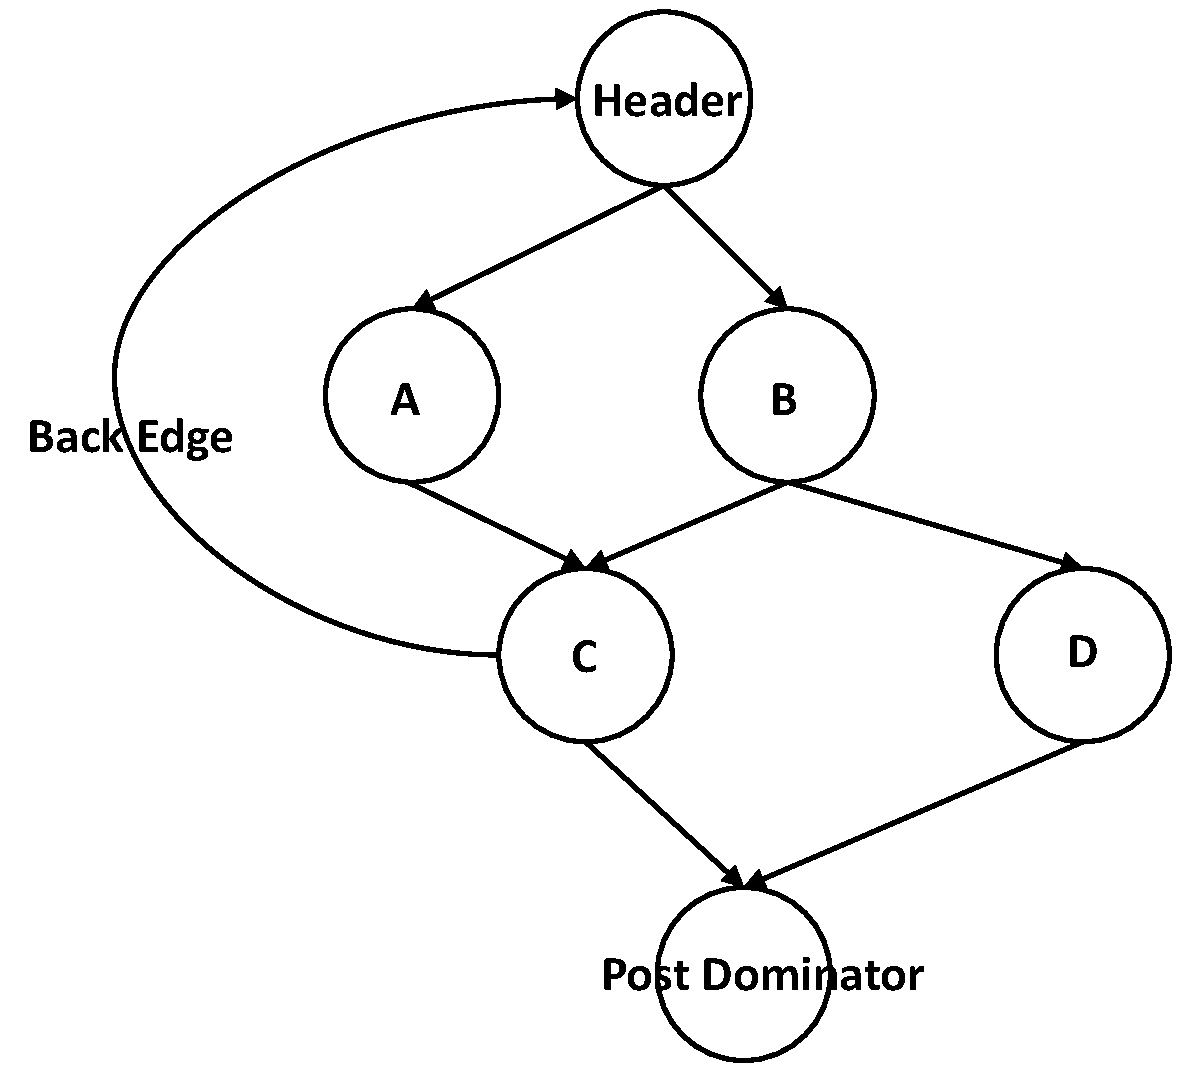
\includegraphics[width=0.7\linewidth]{figures/workless.pdf}
%\caption{Examples for different types of basic blocks inside a loop}
%\label{fig:block_type}
%\end{figure}

\subsubsection{Static Analysis}
\label{sec:s_workless}

\Tool considers two types of instructions as side-effect instructions:
(1) write to heap or global variables;
(2) write to a stack variable, defined outside the loop, and the update value
may be used after the loop. The second condition is checked through liveness
analysis.
\Tool also analyzes all functions called
by a loop directly or indirectly --- a function $F$ that updates variables
defined outside $F$ makes the corresponding call statement in $F$'s
caller a side-effect instruction.
We consider all calls to library functions or through function pointers 
as having side effects, 
unless the library functions are specially marked by us in a white list.
This analysis is complete, but not sound. We may identify side-effect
instructions that are actually not.  

\Tool then categorizes loops into four types.
Given a natural loop $l$, when $l$
contains at least one side-effect instruction along every path that
starts from the loop header and ends at the loop header, it is a 1* loop;
if there exists at least one side-effect instruction inside $l$, but not on
every path,
it is a [0$|$1]* loop; if there is no side-effect instructions inside $l$,
$l$ is either a 0* or a 0*1? loop.
In the last case, \Tool further checks all the loop exit-blocks. If there 
exists an exit-block of $l$ that contains a side-effect instruction and is  
post-dominated by another exit-block of $l$, this is a 0*1? loop.
For example, line 5 in Figure \ref{fig:Mozilla347306} is such an exit block.
Otherwise, $l$ is a 0* loop.

Note that since the 1* pattern contains the least amount of information
about computation \textit{inefficiency}, \Tool will not report a loop's
root-cause type as 1*, if more informative root-cause type is identified 
for this loop (e.g., cross-iteration or cross-loop redundancy).

%TODO Shan will rewrite the next two paragraphs
\subsubsection{Dynamic Monitoring}
\label{sec:d_workless}

Except for 0*, none of the other three type of loops are inefficient for sure.
We need dynamic analysis to figure out what portion of loop iterations are
resultless at run time, which will help decide whether the loop worths fixing.

For a 0*1? loop, since it only generates results in the last iteration, we 
only need to know the total number of loop iterations 
to figure out the loop
\textit{resultful rate}, which we define as the ratio between
the number of iterations with
side effects and the total number of iterations. 
The implementation is straightforward
--- we initialize a local counter to be 0 in the pre-header of the loop; we 
increase the counter by 1 in the loop header to count the number of 
iterations; we dump that counter to log when the loop exits.

For [0$|$1]*, we need to count not only the total number of iterations, but
also the exact number of iterations that execute side-effect instructions
at run time. 
To do that, our instrumentation uses a local boolean variable 
\texttt{HasResult} to represent whether one iteration have side effect or not. 
\texttt{HasResult} is set to \texttt{False} in the loop header, and set to
\texttt{True} after each side-effect instruction. It will be used to help
count the number of side-effect iterations. For performance concerns,
before instrumenting side-effect blocks, we check whether there are 
post-domination relation between each pair of side-effect blocks. 
If both block A and block B are side-effect blocks and block A post-dominates 
block B, we only instrument block A to update \texttt{HasResult}. 

\comment{
We could speed up the above counting using sampling. However, since the 
run-time overhead of the above counting is low, as shown in Section 
\ref{sec:experiment}, our current prototype of \Tool does 
not use sampling for this part of run-time analysis.
}

%\subsubsection{Sampling}
%We calculate the average iteration number 
%and the ratio of working iteration based on a separated 
%process from on-line branch sampling discussed in~\cite{SongOOPSLA2014}.
%We need to instrument the buggy program and re-execute it by using bug-triggering input. 
%In the future, we could design an algorithm to calculate the two resultless metrics 
%based on branch sampling reports to get rid of the extra instrumentation and the extra bad run.   

\comment{
\subsubsection{Limitations}
\label{sec:l_workless}
When callee may have side effect, we will consider it will have side effect in the caller side, 
and do not consider the real execution inside callee. This could bring false negatives, 
because we could miss resultless cases, 
where side effect instructions inside callee do not execute. 
Experiments results in Section~\ref{sec:experiment} show that this is not a big issue, 
since we do not miss any resultless bugs.  

Second, our dynamic instrumentation does not consider concurrent execution of the monitored loop, 
because most of buggy loops we study only execute in one single thread. 
When the monitored loop is executed in multi-thread, like loop marked with omp pragma, we need to synchronize updates to global variables. 
}

\subsection{Redundancy Checker}
\label{sec:redundant}

\subsubsection{Design overview}
To check whether there is redundant computation across different iterations
of one loop instance or across different instances of one static loop, we need
to address several challenges.

\begin{figure}
  \centering
  \lstset{basicstyle=\ttfamily\fontsize{8}{8}\selectfont,
     morekeywords={+},keepspaces=true,numbers=left}
  \mbox{\lstinputlisting[mathescape,boxpos=t]{figures/Apache34464.c}}
  \caption{A cross-loop redundant bug in Apache}
  \label{fig:Apache34464}
\end{figure}

\emph{How to judge redundancy between two iterations/loop-instances?}
Given two iterations (or loop-instances) $i_1$ and $i_2$, since they have 
the same source code, 
a naive, yet expensive, solution is to record and compare the return value of
every memory read conducted by $i_1$ and $i_2$. Two better alternative
solutions are to record and compare only the values written by the
side-effect instructions, such as 
line 9 in Figure~\ref{fig:Mozilla477564},
or read by 
the source instructions\footnote{We define source instructions in a code
region $r$ as a set of memory-read instructions that side-effect
instructions in $r$ depend on and do not depend on any other instructions
inside $r$.}, 
such as source[i] at line 12 of Figure~\ref{fig:Apache34464}.

Among the the above two potential solutions, our design chooses the second one,
because it is
more informative for performance diagnosis 
to track the cause rather than the effect.

\emph{How to handle partial redundancy?}
In practice, redundant loops may be doing largely the same, but not exactly
the same, computation across iterations or loop instances. 
%It is also possible
%TODO define loop instance.
%that only some, instead of all, iterations in a loop are doing redundant
%computation. 
We will discuss how we handle this issue in Section \ref{sec:cal}.



\emph{How to lower the overhead of record-and-compare?}
Even if we only record and compare the values returned by source instructions
the run-time overhead and the log size
could still be large. We will use static analysis and run-time sampling
to lower this time and spatial
overhead 
(Section \ref{sec:inst} and \ref{sec:perf}).
%TODO static analysis alone is not sufficient, because some redundant is
%workload dependent

\emph{How to provide the most suitable fix-strategy suggestion?}
Finally, as discussed in Section \ref{sec:study_ob} and Table \ref{tab:root},
memoization and batching are both common fix strategies for redundant loops.
To pick the right fix strategies,
extra analysis is conducted by \Tool and presented in 
Section \ref{sec:redundant_fix}.

\subsubsection{Identifying source instructions}
\label{sec:dependence}

Informally, we use static analysis to identify a set of 
memory-read instructions that the loop computation depends on. We refer
to these instructions as \textit{source} instructions. The values returned
from them at run-time will be tracked and compared to identify
redundant computation.

Specifically, we first identify side-effect instructions in the loop, as 
discussed in Section \ref{sec:s_workless}; we then conduct static slicing 
from these instructions, considering both control and data
dependency, to identify source instructions.

%TODO How do you handle constant values? I didn't get it.
Our slicing ends when it reaches either a local-variable read conducted
outside the loop or a heap/global-variable read anywhere in the program.
For the latter case, our slicing stops because tracking data-dependency
through heap/global variables is complicated in multi-threaded C/C++
programs. For the former case, 
not including local-variable reads inside the loop can help reduce the
amount of data that needs to be recorded. 
When there are function calls inside the loop,  
we conduct slicing for return values of callees and side-effect instructions
inside callees. 
%In order to reduce the number of memory read we need to record inside callees, 
%we calculate previous writes conducted to the same address for each local-structure read and local-array read. 
%Since local structures and local arrays are mainly used in the declared functions, 
%it is easy to know whether read or write conducted on them are applied to the same address. 
We omit encountered constant values through slicing, because constant values will not influence whether a loop or an iteration is redundant. 


%We conduct slicing to for return values of callees and side-effect instructions
%inside callees. In order to reduce the number of memory read we need to record, 
%we design a GEN-KILL based algorithm to analyze previous writes for read from local structures and arrays 
%inside callees.
%TODO Linhai, I have no idea what you are talking about below
%For a memory read inside a callee function, 
%if its source is a structure or an array declared in the same function, 
%we use a GEN-KILL based algorithm to analyze previous writes for these reads. 
%We do not track previous writes for other memory reads, because it is very difficult to do inter-procedural alias analysis.  

% function() {
%  struct A;
%  A.a = 10;     // place a,
%  if(...)
%  {
%     A.a = 20;  // place b, value defined in place a will be killed, and this place gen a new value
%     print A.a  // A.a will be 20, because only value defined in place a is live 
%  }
%  return A.a;  // there will be memory read here. 
%  //We will do analysis to track where is the previous write for field a of struct A.
%  //The result will be write in place a, and place b
%  //We then conduct dependence analysis for these two writes.
%  //We only do this for read from structure and array declared in the same function. 
% }

The analysis for cross-iteration and cross-loop redundancy analysis is pretty
much the same. The only difference is that, if a memory read instruction 
$i$ in a loop depends on the value returned by instruction $j$ in an earlier
iteration, we stop tracing the dependence at $i$ and consider $i$ as a
source instruction for cross-iteration redundancy analysis, while we continue
the slicing for cross-loop redundancy analysis. 
For example, 
the instruction defining the value of \texttt{i} is the only side-effect instruction 
for the loop at line 12 of Figure~\ref{fig:Apache34464}. 
The source instructions calculated by cross-loop dependence analysis include 
memory read \texttt{source[i]} inside the loop, 
and three values defined outside the loop, 
which represent the initial value of \texttt{i}, the value of \texttt{max} and \texttt{first} respectively. 
In contrast, 
the source instructions calculated by cross-iteration dependence analysis 
include value \texttt{i} defined in previous iteration, 
memory read \texttt{source[i]}, 
and two values defined outside the loop (\texttt{max} and \texttt{first}).  


\comment{
We consider two types of dependence, control dependence and RAW data dependence. 
We build control dependence graph according to the algorithm discussed in~\cite{controldep}. 
If block A is one of ancestors of block B on the control dependence graph, 
we consider all instructions in block B control depend on the branch condition in block A. 
Data dependence is mainly calculated based on instructions' operands. 
We define several types of instrumentation sites. 
The inputs of our dependence analysis are instructions, 
and the output of our dependence analysis is a set of dependent values, 
including instrumentation sites and constant values. 

Before calculating dependence inside the monitored loop, 
we conduct inter-procedural dependence analysis for each function directly called by the loop. 
The formal parameters of each direct callee, memory instructions, 
including load, memcpy, and memmove, 
whose source is not from local structures or arrays, 
and return values of library function calls are instrumentation sites. 
During calculating dependence, 
we consider formal parameter data depend on all real parameter, 
the return value of each call site data depend on return inside the callee function, 
and all instructions inside one callee functions inherit control dependence of all its call site. 

If a direct callee from the monitored loop does not contain recursive function calls, 
we use a three-stage method to solve the infeasible path problem. 
Assume function A is called inside the monitored loop, function A will call function B, 
and function B will call function C. 
We will have a call tree A $\rightarrow$ B $\rightarrow$ C. 
This call tree does not have recursive function calls, so our three-stage method can apply to this case. 
At the first stage, we conduct intra-procedural dependence analysis for each function.  
We consider return values of all call sites as instrumentation sites. 
For example, we consider both the return value of B in A and the return value of C in B as instrumentation sites. 
At the second stage, we process each function bottom-up on the call tree. 
For each call site inside a function, we calculate 
how the return value depend on real parameters based on dependence information inside the callee.
Back to our example, we will process the three functions in order C, B, and A.
When processing function B, we calculate the dependence for the return value of function C 
based on the dependence information inside C and the real parameters of the call site.
At the last stage, we process each function top-down on call tree, 
and calculate dependence for instruction inside a callee function based on information from all its call site. 
At this stage, we will process the three function in the order A, B, and C. 
We update dependence information inside function B, according to control dependence and real parameters of its call site in A. 

We design a Gen-Kill based intra-procedural analysis to 
calculate which previous writes a memory read from local structures and arrays depends on. 
The basic idea is that a memory write will kill all previous writes whose destination address it can cover, 
and the memory write will generate a new write to its destination address. 
Each memory read depends on previous writes whose destination addresses overlap with its source address. 

For the monitored loop, we calculate dependent values for all site-effect instructions, 
including side-effect instructions inside the loop and side-effect instructions inside the callees. 
For cross-loop dependence analysis, instrumentation sites include values defined outside the loop, 
memory reads inside the loop, memory reads not from local structure and arrays inside callees, 
and return values of library function calls. 
For cross-iteration dependent analysis, instrumented sites also include value defined in previous iterations. 
For example, the instruction defining the value of \texttt{i} is the only side-effect instruction 
inside the loop at line 12 in Figure~\ref{fig:Apache34464}. 
After running cross-loop dependence analysis, the dependent values include 
memory read \texttt{source[i]} inside the loop, 
and three values defined outside the loop, 
which represent the initial value of \texttt{i}, the value of \texttt{max} and \texttt{first} respectively. 
After running cross-iteration dependence analysis, 
the dependent value include value \texttt{i} defined in previous iteration, 
memory read \texttt{source[i]}, 
and two values defined outside the loop (\texttt{max} and \texttt{first}).  

}

\subsubsection{Identifying redundant loops}
\label{sec:cal}

After identifying source instructions, we instrument them to record
what values they read from memory
at run time.
%Specifically, we will assign
%a unique ID for each source instruction, and a pair of $<InstID, Value>$
%will be recorded at run time with the execution of a source instruction.
Our trace also includes some delimiters and meta information that allows
trace analysis to differentiate values recorded from different instructions, 
loop
iterations, loop instances, and so on.
%TODO
%All values defined outside the loop is recorded in block O. 
%We record a delimiter, loop instance number and values defined in previous iterations in block H1'.
%Since we only consider redundant iterations from the same loop instance,  
%we do not record values defined outside the loop for cross-iteration redundancy. 



After collecting values returned by source instructions from every iteration
of one or multiple loop instances, we need to process the trace and decide
whether the loops under study contain cross-iteration redundancy or 
cross-loop redundancy. We will first present our high-level algorithms, followed
by the exact implementation in our prototype.

\paragraph{High-level algorithms}
For cross-iteration redundancy, we need to answer two questions. 
First, how to judge whether
two iterations are doing redundant work?
Second, is a (dynamic) loop problematic when it contains only few 
iterations that are
redundant with each other?

Our answer to these two questions stick to one principle: there should be
sufficient amount of redundant computation to make a loop likely root-cause
for a user-perceived performance problem and to make itself worthwhile to
get optimized by the developers. Consequently,
for the first question, \Tool takes a strict 
definition --- only iterations that are doing exactly the same computation are
considered redundant. Since one iteration may not contain too much computation,
a weaker definition here may lead to many false positives. For the 
second question, we believe there should be a threshold. In our current 
prototype,
when the number of distinct iterations is less than half of the total iterations, 
we consider the loop to be cross-iteration redundant. 
%when the number of distinct iterations is less than half of the total iterations 
%iterations/(distinct iterations) = 2

\begin{figure}
  \centering
  \lstset{basicstyle=\ttfamily\fontsize{8}{8}\selectfont,
     morekeywords={+},keepspaces=true}
  \mbox{\lstinputlisting[mathescape,boxpos=t]{figures/Apache37184.java}}
  \caption{A cross-iteration redundant bug in Apache}
  \label{fig:Apache37184}
\end{figure}

For example, Figure~\ref{fig:Apache37184} shows a loop from Apache-Ant that
contains cross-iteration redundancy.
Under the problem triggering input, there are
only few distinct listeners, and most of the
loop iterations in \texttt{fireMessageLoggedEvent}
are doing redundant work. 
%The problem for this bug is that developers say that the performance 
%loss happens in fireMessageLoggedEvent, but in the code I found, function
%messageLogged does not contain anything, and it is an empty function.
%I guess either developers do not have correct understanding of this bug,
%or I did not find the correct codes. 





For cross-loop redundancy, we need to answer similar questions,
especially how to judge whether two loop instances are doing redundant work ---
should they contain exactly the same number of iterations and doing exactly
the same computation in each iteration?
%Second, is a (static) loop problematic when it contains two instances that
%are redundant with each other?

Our answers here are different from our answers above for cross-iteration
redundancy analysis.
We do not require two loop instances to
conduct exactly the same computation to be considered redundant. The rationale
is that a whole loop instance contains a lot of computation, much more than
one iteration in general. Even if only part of its computation
is redundant, it could still be the root-cause of a user-perceived performance
problem and worth developers' attention. 

In fact, in practice, we almost have never seen cases where different loop 
instances are doing exactly the same computation.
For example, Figure~\ref{fig:Mozilla477564} demonstrates a cross-loop redundancy
problem in Mozilla. Here, the
latter instances contain more iterations than previous instances. 
Figure~\ref{fig:Apache34464} shows an example in Apache, 
The inner loop, which starts from line 9,  
searches from the beginning of a string \texttt{sb} for a target sub-string 
\texttt{s}. Since the outer loop, which starts on line 36, appends one 
character to \texttt{sb} in every iteration, every inner loop instance is 
doing computation that is similar, but not exactly the same, 
from its previous instance.


\paragraph{Detailed algorithm implementation}

The implementation of checking cross-iteration redundancy is straightforward.
We will record a sequence of $<InstID, Value>$ pair for every monitored
iteration, with each $InstID$ representing a unique source instruction.
We consider two iterations to be redundant, if their sequences are exactly the
same. To make sure a loop contains sufficient redundant computation, 
we calculate a loop's \textit{cross-iteration redundancy rate} --- dividing 
the total number of iterations in the loop by the number of distinct iterations.
The smaller the rate is, with 1 being the minimum possible value, 
the less cross-iteration redundancy the loop contains.

The implementation of checking cross-loop redundancy goes through several
steps. First, for $k$ dynamic instances of a static loop $L$ that appear
at run time, denoted as $l_1$, $l_2$,
..., $l_k$, we check whether redundancy exists between $l_1$ and $l_2$, 
$l_2$ and $l_3$, and so on. Second, we compute a 
\textit{cross-loop redundancy rate} for $L$
--- dividing the number of redundant pairs by $k-1$.
The smaller the rate is, with 0 being the minimum possible value, the
less cross-loop redundancy $L$ contains.
Here we only check redundancy between consecutive loop instances, because  
checking the redundancy between every pairs of loop
instances is time consuming.

The key of this implementation is
to judge whether two dynamic loop instances $l_1$ and $l_2$ 
are redundant or not.
The challenge is that $l_1$ and $l_2$ may have executed different number of
iterations; in different iteration, a different set of source instructions
may have executed. Therefore, we cannot simply merge values from different
source instructions and iterations together and compare two big data sequence.
Instead, we decide to check the redundancy for each source instruction across
$l_1$ and $l_2$ first, and then use the average \textit{redundancy rate} of
all source instructions as the \textit{cross-loop redundancy rate} between
$l_1$ and $l_2$. 

We calculate the redundancy for one source instruction $I$ by normalizing the
edit-distance between the two sequences of values returned by $I$ in the two
loop instances. The exact formula is the following:

%\[
%\Scale[0.8]{
%min\_dist(SeqA, SeqB) = min(dist(SeqA,SeqB), r\_dist(SeqA, SeqB))
%}
%\]

\[
\Scale[0.8]{
	Redundancy(I) =  \frac{dist(SeqA,SeqB) - (len(SeqA) - len(SeqB))}{len(SeqB)}
}
\]

Here, $SeqA$ and $SeqB$ represent the two value sequences corresponding to $I$
from two loop instances, with $SeqA$ being the longer sequence.
$dist$ means edit distance, and $len$ means the length of a value sequence.
Since the edit distance is at least the length-difference between the
two sequences and at most the length of the longer sequence, we use the 
subtraction and division shown in the formula above to normalize the
redundancy value.

%$r\_dist$ means edit distance after 
%we reverse one sequence. 

%TODO
%We define two configurable thresholds to filter out instance pairs which are both too short, 
%or one is too short compared with the other one.

%TODO
%It is also possible that a source instruction is executed outside the loop.
%We divide values defined outside the loop into several cases.
%Firstly, the value defined outside the loop is only used in the first iteration, 
%and all related values used in following iterations have already been recorded, 
%like the initial value of variable \texttt{n} in Figure~\ref{fig:Mozilla477564}. 
%We omit values defined outside the loop like this.
%Secondly, the value defined outside the loop represent the initial value of an induction variable, 
%like the initial value of variable \texttt{i} in Figure~\ref{fig:Apache34464} 
%for the loop at line 12. We deduce the value sequence of the induction variable 
%based on its initial value and stride, and compare the calculated sequences. 
%Thirdly, the value defined outside the loop only influences side-effect instruction through control dependence, 
%and variables it compares with is not calculated from memory read, 
%like variable \texttt{max} in Figure~\ref{fig:Apache34464}. We think that this type of values only influence how many iterations the loop will execute.
%We calculate redundancy for this type of values by dividing the smaller variable value with the larger one. 
%For all other cases, when the values from two compared instances are the same, redundancy is 1, otherwise, redundancy is 0.

\subsubsection{Dynamic performance optimization: sampling}
\label{sec:inst}

%\begin{figure}[ht]
%\center
%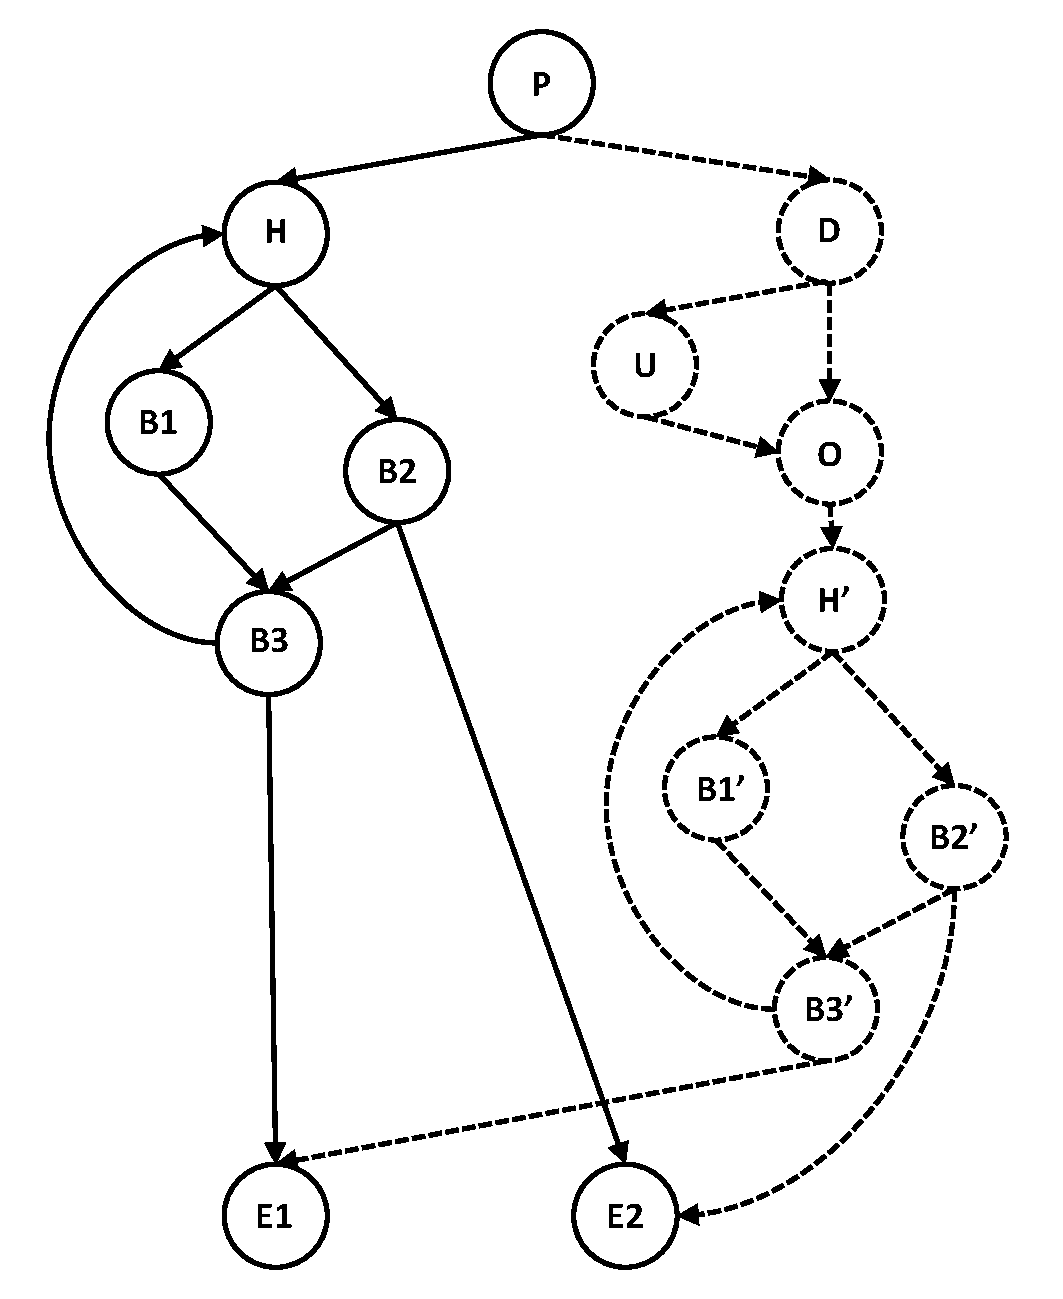
\includegraphics[width=0.7\linewidth]{figures/CL-I}
%\caption{Cross-loop Instrumentation}
%\label{fig:CL-I}
%\end{figure}

Recording values returned by every source instructions would lead to 
huge run-time time. To lower the overhead,
we use random sampling to reduce the number of instructions that we
track at run time. Due to the repetitive nature of performance bugs,
we will still be able to recognize redundant 
computation as long as the sampling rate is not too sparse (we will evaluate
this in Section \ref{sec:experiment}). 
Our sampling scheme requires almost no changes to our redundancy 
identification algorithm discussed in Section \ref{sec:cal}.


%Another observation, which can also be demonstrated by examples shown in Figure~\ref{fig:Mozilla477564} and Figure~\ref{fig:Apache34464}, 
%is that two consecutive loop instances are good targets to compare.

%There are two possible reasons for cross-iteration redundancy. 
%The first one is loop-invariant computation, which can be identified statically, 
%and it is the target for traditional compiler optimization. 
%The second one is repetitive processed elements, like GCC\#27733 shown in Figure~\ref{fig:GCC27733}. 
%When processed elements are repetitive, the computation conducted by different iterations is exactly the same. 
%If we compare a pair of iterations, we may fail to observe redundancy. 
%For cross-iteration redundancy, we randomly sample iterations, 
%and compare distinct computation number with the total number of sampled iterations. 

\paragraph{Cross-iteration redundancy analysis}
Our high-level sampling strategy is straightforward:
randomly decide at the
beginning of every iteration whether to track the values returned by
source instructions in this iteration.

The implementation is similar with previous sampling work 
\cite{liblit03,liblit05}.
Specifically, we create a clone of the original
loop iteration code, including functions called by the loop directly or
indirectly, and insert value-recording instructions along the
cloned copy. 
We then insert a code snippet that conducts random decision to
the beginning of a loop iteration. 
Two variables \texttt{CurrentID}, which is initialized as 0, 
and \texttt{NextSampleID}, which is initialized by a random integer, 
are maintained
in this code snippet. \texttt{CurrentID} is increased by 1
for each iteration. When it matches \texttt{NextSampleID}, the control
flow jumps to the value-recording clone of the loop iteration and the 
\texttt{NextSampleID} is increased by a random value. Different sampling
sparsity setting will determine the range from which the random value is
generated.

%\begin{figure}
%\center
%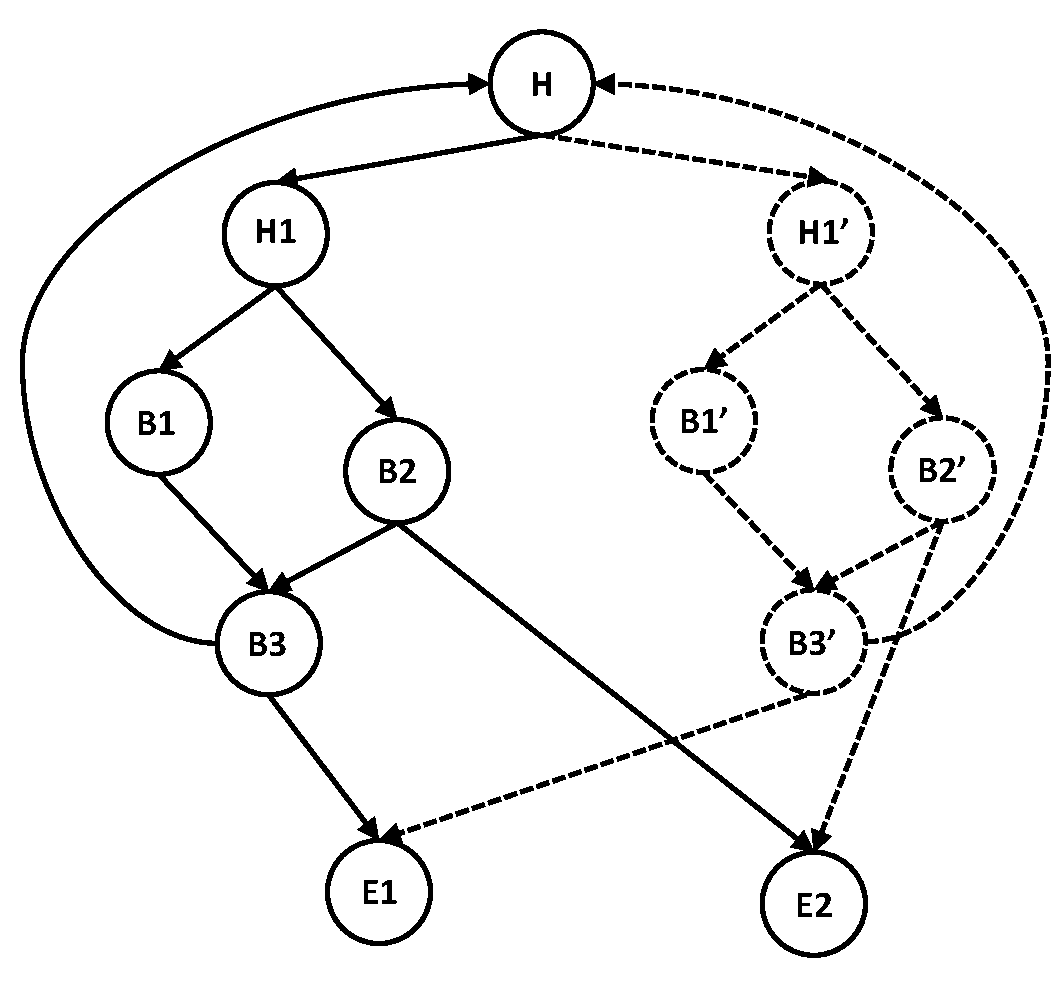
\includegraphics[width=0.7\linewidth]{figures/CI-I}
%\caption{Cross-iteration Instrumentation}
%\label{fig:CI-I}
%\end{figure}

\paragraph{Cross-loop redundancy analysis} 
At high level, we randomly decide at the beginning
of every loop instance whether to track values for this instance. 
Since we will need to compare two consecutive loop
instances for redundancy, once we decide to sample one loop instance, we will
make sure to sample the immediately next loop instance too.
The implementation is straightforward by cloning the whole loop and making
sampling decisions in the loop pre-headers.
%; (2)
%sampling is conducted when \texttt{CurrentID} equals either
%\texttt{NextSampleID} or \texttt{NextSampleID}$+1$, with \texttt{NextSampleID}
%increased by a random value in the latter case.

%TODO
%For each monitored memmove or memcpy instruction, 
%we record its ID, the length of accessed memory, 
%and the content of the accessed memory. 



%\paragraph{Handling recursive functions}
%We also conduct sampling to our redundancy analysis for recursive functions.
%For a recursive function, we first create an instrumented clone copy of 
%the whole function body.
%We then add a sampling-control code snippet at the entry point of the function,
%where \texttt{CurrentID} and \texttt{NextSampleID} are maintained to decide
%whether to execute the original function body or the instrumented 
%value-recording clone copy.
%We also create clones for all the callee functions of the recursive function
%under study, so that the sampling decision can be correctly conducted
%throughout the call chain.

\subsubsection{Static analysis for performance optimization}
\label{sec:perf}

We conduct a series of static analysis to reduce the number of instructions we 
need to monitor. 

First, we identify and avoid monitoring memory reads whose return values can be 
statically proved to
not change throughout one loop instance (i.e., for cross-iteration
redundancy analysis) or multiple loop instances (i.e., for cross-loop redundancy
analysis). Since we implement \Tool at LLVM byte-code level, a major part of this
analysis is already done by LLVM, which lifts loop-invariant memory
accesses out of loops. The only extra analysis we did is to 
prune memory reads whose reading address is loop invariant, and there are no writes 
inside the loop which are possibly conducted on the same address. 
For example, the read address of \texttt{aNode.localName} and \texttt{aNode.namespaceURI}
in Figure~\ref{fig:Mozilla477564} is loop-invariant, and there are no write conducted 
on the same address. We do not need to record these two memory read. 
%It is easy to lift read from local variable outside the loop. 
%Compiler is conservative to move read, which may cause exception, outside the loop.
%I think this part of analysis is to prune memory read which is invariant, but unsafe to be moved out by compiler. 
%llvm is very conservative to move memory read from array/structure/global variable/heap variable
%outside the loop.
%what we do is if the read address is loop invariant, and there are no other write possibly 
%write to the same place, we will not record the memory read.

%TODO: Linhai, I don't understand your original writing. Pls rephrase, and provide
%an toy example.
%For each monitored memory read, we use loop-invariant analysis to identify 
%whether the read address is loop-invariant. 
%If the address is invariant, and there are no memory writes whose addresses 
%may/must alias to the read address, we will not instrument the memory read.

%ANSWER:
%while(i=lower[j]; a[i]<100 & i<upper[j]; i++); 
%The memory read upper[j] is conducted in each iteration.
%The read address upper+j is loop-invariant. If there is not write to the same
%address, the read is also loop-invariant, and we do not need to record the memory read.
%we conduct alias analysis, and analysis whether there are memory writes, whose
%address may/must alias to the read address. 

Second, we identify and avoid monitoring some memory reads whose return values 
can be statically proved to be different throughout one loop instance in 
cross-iteration redundancy analysis.
Specifically, for read on loop induction variable, such as i for loop at line 12 of Figure~\ref{fig:Apache34464}, 
%Specifically, reading of loop induction 
%variables, such as XXX, are always identified as source instructions in % variable i for loop at line 12
%cross-iteration redundancy analysis; 
we also know for sure that their return
values are different in different iterations. 
If source instructions include read on loop induction variables, we know that 
there could not be cross-iteration redundancy. 
We use scalar evolution analysis
provided by LLVM to identify induction variables and avoid tracking their
values.
%induction variables are not always identified as source instructions.
%it could be possible that side-effect instructions do not depend on induction variables.
%for example, side-effect instruction may only depend on array content, and array index 
%will not be source instructions

%TODO: Linhai, I find it hard to believe that consider "there will not be
%cross-iteration redundancy simply because induction variable is in the 
%dependent set. Really? The input workload itself could be repetitive, and hence
%could still deserve monitoring, right? 
%


%ANSWER: this is true according to how we calculate cross-iteration redundancy.
%We only consider iteration from the same loop instance.
%induction variable will be changed in each iteration by a fix constant, so
%the value of induction variable will be different from each other in each iteration of the same loop instance. 
%The case you mention is 
%for(i=0; i < 10; i ++) {
%  c = A[i]; 
%   ...   // all other computation only depend on c        
% }
%Our dependence analysis will report the memory read A[i] as dependent value, not i.
%If the content of A is repetitive, we will identify cross-iteration redundancy.
 
%For cross-iteration instrumentation, we use scalar evolution analysis to identify 
%whether there are induction variables in the dependent value set. 
%A induction variable will be increased or decreased by a fix amount in each loop iteration. 
%If there are induction variable inside the dependent value set, 
%we know that there will not be cross-iteration redundancy. 


Third, sometimes we only record the memory-address range of a sequence of memory
read, instead of the value returned by every read, in cross-loop redundancy
analysis. 
The loop at line 12 in Figure~\ref{fig:Apache34464} shows an example.
The content of array \texttt{source} is never modified
throughout the outer-loop, which starts 
at line 12 in the Figure~\ref{fig:Apache34464}.
%We do not have the static analysis to prove the content of array does not change.
%for source[i] for the loop at line 12, we only need to record source, initial value of i and final value of i. 
%TODO
%Do you really do analysis to prove that the source array is not changed?
%ANSWER
%Shan, I do not have invariant analysis to prove the the source array is not changed.
%I remove that part of writing in the last version I sent to you. 
%It is very difficult to implement the invariant analysis.
%I plan to discuss this in limitation part of this section, and say that this could bring false positives.
%There are reasons why I feel it is too difficult to implement the invariant analysis:
%1. it is difficult to find the range (the outer loop) to apply the analysis.
%assume we have loopA, loopB and loopC. loopA contains loopB, and loopB contains loopC. 
%we are analyzing loopC. It could be possible that loopB only execute 1 or 2 iterations, and loopA is the real outer loop
%2. It is very difficult to prove that there is no other loop inside the outer loop which does not write to the same array.
%There could be cases like:
% for(i = 0; i < 10; i++)
%   func(&(A[i]));
% func will write to its parameter.
Therefore, to check whether different inner loop instances read similar
sequence of array data, we only need to record the starting and 
ending array index touched by each inner loop, significantly reduce the 
monitoring overhead. To accomplish this optimization, we again leverage
the scalar evolution analysis provided by LLVM. The scalar evolution analysis
tells us whether the address of a memory read instruction
is a loop induction variable. For example, the address for memory read \texttt{source[i]} is added by one in each loop iteration,
so it is a loop induction variable. 
From the scalar evolution analysis, we know that the starting address is \texttt{source} plus the initial value of \texttt{i}, and the ending address
is source plus the ending value of \texttt{i}.  
%TODO Linhai, I don't understand your original text. The address is 
%source+i; loop induction variable is i. What do you mean by "the read address
%is an induction variable"? Please rewrite.

%ANSWER
%Shan, both source + i and i are induction variables, because both of them 
%will be added by 1 in each iteration. The only difference between these two 
%are their initial values.
%For cross-loop redundant bugs, we also rely on scalar evolution analysis to identify whether the read address
%is an induction variable for each monitored read instruction. 


\subsubsection{Fix strategy recommendation}
\label{sec:redundant_fix}
As discussed in Section \ref{sec:tax_study}, extra analysis is needed to
decide whether batching or memoization should be suggested to fix a 
loop that conducts redundant computation.

For cross-iteration redundancy, batching is often used towards
batching I/O related operations, based on our empirical study. 
Therefore, we treat I/O related redundancy separately.
Specifically, when the only side effect of a loop is I/O operations
and the same statement(s) is executed in every loop iteration, we report this
as I/O related redundancy problem and suggest batching as a potential fix
strategy. 

For cross-loop redundancy, whether to use memoization or batching often
depends on which strategy is cheaper to use. \Tool uses a simple
heuristic. If 
the side effect of each loop instance is to update 
a constant number of memory locations, like the 
buggy loop in Figure~\ref{fig:Mozilla477564} and Figure~\ref{fig:Apache34464}, 
we recommend memoization. Instead, if the side effect is updating 
an sequence of memory locations, with the number of locations increasing
with the workload, memoization is unlikely to help save much computation.

%we xxx
%TODO

%%if side effect of the loop is to define several scalar value used outside the loop, we recommend memoization.
%%if side effect is to write to distinct memory address or conduct system call, 
%%we recommend batch



\section{Assessment of Root-Cause Taxonomy}
\label{sec:eval_taxonomy}

%\input section/tab_appbug
\input section/tab_root

\subsection{Methodology}

\comment{
Previous work \cite{PerfBug,SongOOPSLA2014} studied the on-line bug
databases of five representative open-source software projects:
(1) Apache suite, including HTTPD web server written in C/C++,
TomCat server written in Java, and Ant build management tool in Java;
(2) Chromium Google Chrome browser in C/C++;
(3) GCC compiler in C/C++;
(4) Mozilla web browser and
Email client in C/C++ and JavaScript; 
(5) MySQL database server in C/C++.
Through a mix of random sampling and 
manual inspection, they 
found 65 performance problems that are perceived and reported by users. 
Among these 65 problems, 45 are related to inefficient loops and 
hence are the target of the study 
here.
}

Our previous work \cite{PerfBug,SongOOPSLA2014} studied the on-line bug
databases of five representative open-source software projects:
(1) Apache suite, including HTTPD web server written in C/C++,
TomCat server written in Java, and Ant build management tool in Java;
(2) Chromium Google Chrome browser in C/C++;
(3) GCC compiler suite in C/C++;
(4) Mozilla suite, including Firefox web browser and Thunderbird
Email client in C/C++ and JavaScript; 
(5) MySQL database server in C/C++.
{\color{red} By manually inspecting a set of randomly sampled bug reports,
previous work identified 
65 performance problems that are perceived and reported by users~\cite{SongOOPSLA2014}.}  
Among these 65 problems, 45 problems are related to inefficient loops and 
hence are the target of the study
here.

\comment{
\footnote{The definition of ``loop-related'' in this paper is a little
bit broader than earlier paper~\cite{SongOOPSLA2014}, which only considers
43 problems as loop-related. }.
More details can be found in previous papers that collected
these bugs. 
}

\subsection{Assessment}
\label{sec:study_ob}

\comment{
\begin{table*}[tb!]
%\begin{adjustwidth}{-.5in}{-.5in}
\small
\centering
{
\begin{tabular}{|lcccccc|}
\hline
&Apache&Chrome&GCC&Mozilla&MySQL&Total\\
\hline
Total \# of loop bugs & 11 & 4 & 8 & 12 & 10 & 45 \\
\hline
\multicolumn{1}{|l}{Cross-{\bf iteration} Redundancy}
&7&1&2&1&1&12\\
\multicolumn{1}{|l}{ Cross-{\bf loop} Redundancy}
&3&0&2&2&2&9\\
\multicolumn{1}{|l}{ {\bf 0*} Resultless}
&0&0&0&0&0&0\\
\multicolumn{1}{|l}{ {\bf 0*1?} Resultless}
&0&0&0&2&3&5\\
\multicolumn{1}{|l}{{\bf [0$|$1]*} Resultless}
&0&1&1&1&1&4\\
\multicolumn{1}{|l}{{\bf 1*} Resultless}
&1&2&3&6&3&15\\
%&0&2&0&5&0&7&B(4)$|$S(3)\\
%&1&0&3&1&3&8&\\
  %MySQL15811 is moved from 1* to here; consider it as fixed by M
%\hline
%\multicolumn{8}{|c|}{ \# of {\textit {Other}} bugs}\\
%\multicolumn{1}{|l}{Not in above categories}
\hline
\end{tabular}
}
%\end{adjustwidth}
\caption{Number of bugs in each root-cause category. 
}
\label{tab:root}
\end{table*}
}



\comment{
\def\cca#1{\cellcolor{black!#10}\ifnum #1>5\color{white}\fi{#1}}
%For ranges 0-10, multiply by 10 by adding 0 after #1
\begin{table}[tb!]
%\begin{adjustwidth}{-.5in}{-.5in}
\small
\centering
{
\begin{tabular}{lcccccc}
%\hline
                                 &{\bf 0*}    & {\bf 0*1?} & {\bf [0$|$1]*}   & {\bf 1*} & {\bf C-I}  & {\bf C-L} \\
%\hline
 B                               & \cca{0}    & \cca{0}    & \cca{0}          & \cca{4}  & \cca{4}     & \cca{4}   \\
%\hline
 M                               & \cca{0}    & \cca{0}    & \cca{0}          & \cca{0}  & \cca{7}     & \cca{5}   \\
 S                               & \cca{0}    & \cca{1}    & \cca{4}          & \cca{4}  & \cca{0}     & \cca{0}   \\
 C                               & \cca{0}    & \cca{4}    & \cca{0}          & \cca{0}  & \cca{0}     & \cca{0}   \\
 O                               & \cca{0}    & \cca{0}    & \cca{0}          & \cca{7}  & \cca{1}     & \cca{0}   \\
%\hline

\end{tabular}
}
%\end{adjustwidth}
\caption{Number of bugs fixed by each strategy:
B(atching),  
M(emoization), 
S(kipping the loop),
C(hange the data structure), and O(thers). 
``C-I'': cross- iteration redundancy. 
``C-L'': cross-loop redundancy. 
}
\label{tab:correlation}
\end{table}
}


\textit{Coverage:}
As shown in Table \ref{tab:root}, 
our taxonomy does cover all inefficient loops under study. 
Resultless loops are about as common as redundant loops
(24 vs. 21).
Not surprisingly, 0* loops
are rare in mature software. 
%In fact, no bugs in this
%benchmark suite belong to this category.
All other root-cause sub-categories are well represented.


\textit{Actionability:}
As shown in Table \ref{tab:root}, 
the root-cause categories in our taxonomy are well correlated with
fix strategies.
This indicates that our taxonomy is actionable --- once the root cause
is identified, developers roughly know how to fix.
For example, 
almost all 0*1? resultless loops are fixed by data-structure changes;
all [0$|$1]* resultless loops are
fixed by conditionally skipping the loop;
almost all redundant loops are fixed either by 
memoization or batching. 
The only problem is that there are no silver bullets for fixing 1* loops.
%all inefficient loops with xx root cause are fixed by xxx.
%xxx

\textit{Generality:}
The root-cause categories in our taxonomy are designed to be 
generic. Table \ref{tab:root} also shows that these categories 
each appears in multiple
application in our study. The only exception is $0^*$-resultless, which
never appears. 


In summary, the study above informally demonstrates that our taxonomy
is suitable to guide our design of \Tool.
%chances to satisfy the coverage and accuracy requirements of performance 
%diagnosis.
%
%TODO even for the other, there are things we could do ...



\section{Evaluation of \Tool}
\label{sec:experiment}

\subsection{Methodology}
\label{sec:result_meth}
%Please discuss the potential usage scenarios of \Tool
%How you will use it together with other tools 

\input section/tab_benchmarks

\paragraph{Implementation and Platform}
We implement \Tool in LLVM-3.4.2 \cite{llvm}, and conduct our
%Our implementation consists of 17654 lines of C++ code, 
%with 4748 for instrumenter, 674 for resultless analysis, 
%5802 for redundancy analysis, 
%and the remaining 6430 for common utilities. 
experiments on a i7-960 machine, with Linux 3.11 kernel. 

\paragraph{Benchmarks}
Note that \Tool is a tool that helps diagnose performance problems that
have already manifested, not a detection tool that can help predict not-yet-manifested
problems. Consequently, our benchmarks are performance problems that have already
happened in real world, and we will reproduce these problems to evaluate \Tool.
To conduct a thorough evaluation, we use
benchmarks from two sources.

First, we evaluate \Tool on 18 out of the 45 bugs listed in Table \ref{tab:root}. 
Among these 18, seven are extracted from Java or JavaScript
programs and re-implemented in C++, as \Tool currently only handles C/C++
programs; one is extracted from a very old version of Mozilla.
%These 18 bugs include all the benchmarks used in the recent
%statistical performance debugging work~\cite{SongOOPSLA2014}.
The extraction is conducted by XXX.
We did not use the remaining 27 bugs listed in Table \ref{tab:root}
as benchmarks, 
either because they depend on special hardware/software environment
or because they involve too complex data structures to extract XXX. 
Overall, these 18 bugs cover a wide variety of inefficiency root causes, as 
shown in Table~\ref{tab:benchmarks}. 

Second, we evaluate \Tool on 21 out of the xx bugs in the benchmark
suite of Toddler \cite{Alabama}.
All of these bugs come from Java programs. We extract XXX (how did you
extract exactly?) and re-implement in C++. Each extracted benchmark 
contains 4--5 loops (how come you always have 4--5 loops??XXX). 
Note that, Toddler focuses on inefficient nested loops, and its
benchmark bugs only cover two types of inefficiency root causes,
as shown in Table \ref{tab:benchmarks}.
We use Toddler benchmark suite because it provides a larget set of
repeatable inefficient loop problems. 


\paragraph{Metrics}
Our experiments are designed to evaluate \Tool from three main aspects:
(1) 
\textit{Coverage}. Given our benchmark suite that covers a wide variety
of real-world root causes, can \Tool identify all those root causes?
(2)
\textit{Accuracy}. 
When analyzing non-buggy loops, will \Tool generate any false positives?
(3) 
\textit{Performance}.
What is the run-time overhead of \Tool?

\paragraph{Evaluation settings}
Our evaluation uses existing statistical performance diagnosis
tool \cite{SongOOPSLA2014} to process a performance problem and identify 
one or a few suspicious loops for \Tool to analyze.
For 14 out of the 18 benchmarks, statistical debugging identifies the
real root-cause loop as the most suspicious loop. For the remaining
benchmarks, the real root-cause loops are ranked number 2, 2, 4, and 10.
%Overall, we believe future tools can accurately identify the most one or a couple
%of suspicious loops.
XXX (what can we say about Toddler benchmark set here?)

\input section/tab_cover

To evaluate the coverage, accuracy, and performance of \Tool, we mainly conduct
three sets of evaluation. First, we apply \Tool to the real root-cause loop to
see if \Tool can correctly identify the root-cause category and provide
correct fix-strategy suggestion. Second, we apply
statistical performance debugging \cite{SongOOPSLA2014} to all our benchmarks
and apply \Tool to the top 5 ranked loops\footnote{Some extracted benchmarks
have fewer than 5 loops. We simply apply \Tool to all loops in these cases.}
to see how accurate \Tool is. Third, we evaluate the run-time performance of
applying \Tool to the real root-cause loop. 
 
For all benchmarks we use, real-world
users have provided at least one problem-triggering input in their on-line 
bug bugs. We use these inputs in our run-time analysis.

As discussed in Section \ref{sec:design}, our analysis contains 
several configurable thresholds. In our evaluation,
we use 0.001 as the \textit{resultful rate} threshold for identifying
0*1? 
%loops, 0.01 as the \textit{resultful rate} threshold for identifying 
and [0$|$1]* resultless loops; we use 
0.5 as the \textit{redundancy rate} threshold for identifying redundant loops.
%, and 
%2 as the \textit{cross-iteration redundancy rate} (i.e., 
%the number of distinct iterations is less than half of the total iterations).

All the analysis and performance results presented below regarding
cross-loop analysis is obtained using $1/100$ sampling rate; all the
results regarding cross-iteration analysis is obtained using $1/1000$ sampling
rate. We use sparser sampling rate in the latter case, because there tend to
be more loop iterations than loop instances.
All our diagnosis results require only \textbf{one} run under the 
problem-triggering input.

More discussions about all the parameters/thresholds presented above, including
how to set them and how sensitive they are, are discussed in Section
\ref{sec:sensi}. 

\subsection{Coverage Results}
\label{sec:coverage}
Overall, \Tool provides good diagnosis coverage, as shown in Table~\ref{tab:cover}. 
\Tool identifies the correct root cause for \textbf{all} \allbugs benchmarks, and 
suggests fix strategies that exactly match what developers took in practice
for 33 out of \allbugs cases. 

The six cases where the fix strategy suggested by \Tool does not match that of 
developers fall into three categories.
First, the fix strategy taken by developers is a subset of what suggested by 
\Tool.
For MySQL\#27287 and Apache\#53622, the root-cause loop
is both cross-loop redundant and 0*1? inefficient. \Tool suggests both changing
data structures and memoization as fix strategies. In practice, the developers
only changed the data structure, which eliminated both types of inefficiency,
in case of MySQL\#27287, or the main type of inefficiency, in case of Apache\#53622.

Second, the fix strategy taken by developers is a superset of what suggested by
\Tool.
In Collections bugs \#407, \#408, and \#425, XXX.

Third, \Tool cannot suggest fix strategy for 1* loops.
For GCC\#12322, \Tool correctly tells that the loop under study
does not contain any form of inefficiency and produce results in every 
iteration, and hence fails to suggest any fix strategy. In practice, GCC
developers decide to skip the loop, which will cause some programs compiled by
GCC
to be less performance-optimal than before. However, GCC developers feel
that it is worthwhile considering the slow-down caused by the original loop.

\subsection{Accuracy Results}
\label{sec:result_acc}

\input section/tab_top5

As shown in Table \ref{tab:top5}, \Tool is accurate, having 0 real
false positive and 23 benign false positives for all the top 5 loops
of the \allbugs benchmarks.

Here, benign false positives mean that the \Tool analysis result is true ---
some loops are indeed cross-iteration/loop redundant or indeed producing
results in only a small portion of all the iterations. However, those
problems are \textit{not} fixed by developers in their performance patches. 

There are several reasons for these benign performance problems. 
The main reason is that they are not the main contributor to the 
performance problem perceived by the users. This happens to 11 out of the
13 benign cases (XXX subject to change XXX). 
In fact, this is not really a problem for \Tool in 
real usage scenarios, because statistical debugging can accurately
tell that these loops are not top contributors to the performance
problems.
Two cases happen when fixing the 
identified redundant/resultless problems
are very difficult and hence developers decide not to fix them.
The remaining cases XXX.


The accuracy of \Tool benefits from its run-time analysis.
For example, there are 7 (XXX to change XXX) benchmarks in total that each contains
a loop that generates side effect only
in its last iteration. Without run-time information, \Tool would judge
all of them as inefficient (0*1? resultless). Fortunately,
\Tool run-time counts the total number of iterations and
correctly identifies 3 (XXX to change XXX) of them as truly inefficient and severe enough
to cause the corresponding performance problem.

\Tool can also help improve the accuracy of statistical debugging in
identifying which loop is the root-cause loop.
For example, the real root-cause loop of Apache\#34464 and GCC\#46401 both
rank number two by the statistical performance diagnosis tool.
Fortunately,
\Tool can tell that the number one loops in both cases do not contain
any form of inefficiency, resultless or redundancy. 

\subsection{Performance}
\label{sec:result_perf}

\begin{table}
  \centering
  \scriptsize
  \newcommand{\Yes}[1]{\checkmark{}$_#1$}
  \newcommand{\No}[0]{-}
  \begin{tabular}{lccccc}
    \toprule
	    & \multicolumn{3}{c}{\Tool w/ optimization} & \multicolumn{2}{c}{w/o optimization} \\
     \cmidrule(lr){2-4}
     \cmidrule(lr){5-6}
     {\bf BugID}  & {\bf Resultless}  &  {\bf C-L R. } & {\bf C-I R. }  & {\bf C-L R.}  & {\bf C-I R. } \\
    \midrule
    Mozilla347306 &  1.07\%           &  22.40\%       &  10.17\%       & 304.37{\bf X} & 468.74{\bf X} \\ 
    Mozilla416628 &  0.80\%           &  4.10\%        &  2.99\%        & 567.51{\bf X} & 85.6{\bf X} \\
    \midrule
     MySQL27287   & $<$0.01\%           &   1.66\%       &   -            & 109.55{\bf X} & 352.07{\bf X} \\
     MySQL15811   &  -                &   0.03\%       &   -            & 227.04{\bf X} & 424.44{\bf X} \\
    \midrule
      GCC46401    & 3.12\%         & 3.80\%            &  5.95\%        & 21.07{\bf X}  & 38.44{\bf X}\\ 
      GCC1687     & -              & /                 &  $<$0.01\%       &   /           & 142.29{\bf X} \\
      GCC27733    & $<$0.01\%        & /                 &  4.73\%        &   /           & 17.41{\bf X}     \\
      GCC8805     & -              & $<$0.01\%           & $<$0.01\%        & 2.22{\bf X}   &  3.52{\bf X}\\
      GCC21430    & -              & 5.46\%            &   0.69\%       & 107.20{\bf X} & 159.89{\bf X} \\
      GCC12322    & -              & 1.75\%            &  $<$0.01\%       & 21.07{\bf X}  & 38.44{\bf X} \\
   \bottomrule
   \end{tabular}
  %\nocaptionrule
  \caption{Run-time overhead of applying \Tool to the buggy loop
    (only non-extracted benchmarks are shown). 
  -: dynamic analysis is not needed;
  /: not applicable.}
  \label{tab:performance}
\end{table}


As shown in Table \ref{tab:performance}, 
the performance of \Tool is good. The overhead is consistently under or around 5\% 
except for one benchmark, Mozilla\#347306. We believe \Tool is promising for potential production
run usage.
We can easily further lower the overhead through sparser sampling.
As we will discuss later, 
the current diagnosis results are obtained by running the
program only \textbf{once} under the problem-triggering workload.
If we use sparser sampling, more failure runs will be needed to obtain good
diagnosis results.

As we can also see from the table, our performance optimization discussed in 
Section \ref{sec:inst} and \ref{sec:perf} has helped.

The performance benefit of sampling is huge.
Without sampling, even with all the static optimization, redundancy
analysis lead to over 100X slowdown for five benchmarks.

The benefit of static optimization is also non-trivial. 
For example, for MySQL\#15811 and MySQL\#27287, static analysis alone can
judge that they do not contain cross-iteration redundancy: the computation of 
each iteration depends on loop induction variables, which are naturally different
in different iterations. Consequently, run-time overhead is completely
eliminated for these two benchmarks.
As another example, the buggy loops of MySQL\#27287 and MySQL\#15811 access 
arrays. 
After changing to tracking the initial and ending memory-access addresses
of the array, instead of the content of the whole array accesses,
the overhead is reduced from 11.77\% to 1.66\% for MySQL\#27287, 
and from 20.46\% to 0.03\% for MySQL\#15811 respectively 
(sampling is conducted consistently here). 

\subsection{Parameter Setting and Sensitivity}
\label{sec:sensi}
\paragraph{Sampling rates}
We have tried different sampling rates for redundancy analysis.
Intuitively, sparser sampling leads to lower overhead but worse diagnosis
results. Due to space constraints, we briefly summarize the results below.

When we lower the sampling rate from 1/100 to 1/1000 
in cross-loop redundancy analysis,
among all the benchmarks in Table \ref{tab:performance},
Mozilla\#347306 still incurs the largest overhead (0.49\%). 
The diagnosis results remain the same for all but
GCC\#12322, where too few samples are available
to judge redundancy.

When we lower the sampling rate from 1/1000 to 1/10000
in cross-iteration redundancy analysis,
among all the benchmarks in Table \ref{tab:performance},
Mozilla\#347306 has the largest overhead (4.47\%). 
%In fact, Mozilla347306 is the only one whose overhead is larger than 2\%. 
The diagnosis results remain 
the same for all but GCC\#12322.
%If we increase the sampling rate to 1/100, we will 
%have two benchmarks whose overhead is larger than 30\%.

\paragraph{Resultful and redundancy rate}
Since the severity of resultless and redundant loops depends on
workload, it is natural that \Tool uses two thresholds in its diagnosis.
In fact, the diagnosis results are largely insensitive to the threshold
setting. For example, the results would remain the same when
changing the redundancy rate threshold from 0.5 to any value between about
0.1 and 0.66. We will have 1 more false negative and 1 fewer benign false positive, 
when the rate is 0.7. The trend is similar for resultless
loop checking. 
XXX

Our default setting %is obtained based on our experience
should work for many problems.
Developers can adjust these thresholds. 
They can even get rid of thresholds, and only
use the raw values of resultful/redundancy rates to understand
the absolute and relative (in)efficiency nature of suspicious 
loops. Based on our experiments, the difference between efficient and inefficient
loops is usually obvious, based on these rates.

\subsection{Comparison with other tools}
XXXXXX

\section{Related Works}
\label{sec:related}

\subsection{Performance Diagnosis}
Profilers are the most commonly used tools that help developers understand
performance
\cite{Zaparanuks:2012:AP:2254064.2254074,Coppa:2012:IP:2254064.2254076,
D'Elia:2011:MHC:1993498.1993559, 
Mytkowicz:2010:EAJ:1806596.1806618,
Ravindranath:2012:AMA:2387880.2387891,
Jovic:2011:CMY:2048066.2048081,IntroPerf}.
Different from our work, profiling aims to tell where 
computation resources are spent, 
not where and why computation resources are wasted. 
The root cause code region of a performance problem often is not inside
the top-ranked function in the profiling result \cite{SongOOPSLA2014}.
Even if it is, developers still need to spend a lot of effort to understand
whether and what kind of computation inefficiency exists.

Recently, tools that go beyond profiling and provide more automated analysis
have been proposed.
StackMine~\cite{Han:2012:PDL:2337223.2337241} can
identify slow call-stack patterns inside event handlers. The work by
\citet{TaoAsplos2014} analyzes system traces to understand 
performance impact propagation and 
causality relationship among different system components. 
X-ray~\cite{Attariyan:2012:XAR:2387880.2387910} helps identify inputs
or configuration entries that are most responsible for performance problems.
Although these techniques are all very useful, 
they target different problems from \Tool. \Tool targets 
inefficient loops, a common
inefficiency problem that contributes to
about two thirds of real-world user-perceived performance problems studied
by previous work \cite{SongOOPSLA2014}, and tries to pin-point the exact
root cause and provide fix-strategy suggestions.

\Tool is most related to
the recent statistical performance debugging work
\citep{SongOOPSLA2014}, both trying to identify source-code level root causes
for user-perceived performance problems. 
This previous work identifies which loop is most correlated with 
a performance symptom through statistical analysis, 
but cannot answer whether or 
what type of inefficiency this loop contains.
\Tool complements it by
providing detailed root cause information and fix strategy suggestions through
program analysis. 

\subsection{Performance Bug Detection}

Many dynamic and static analysis tools have been built to detect different
types of performance problems, such as 
run-time bloat~\cite{Dufour:2008:STC:1453101.1453111, Xu:2009:GFP:1542476.1542523, Xu:2010:DIC:1806596.1806616}, 
low-utility data structures~\cite{Xu:2010:FLD:1806596.1806617}, 
cacheable data~\cite{Cachetor}, false sharing in
multi-thread programs~\cite{Liu:2011:SPD:2048066.2048070},
inefficient nested loops~\cite{Alabama},
loops with unnecessary iterations~\cite{CARAMEL,IsilDillig.PLDI15},
input-dependent loops~\cite{xiao13:context}, and others. 
%Some static tools \cite{PerfBug} identify performance defects that violate
%specific efficiency rules, often related to API usage. 

As discussed in 
Section \ref{sec:intro}, these tools are all useful in improving software
performance, but are not suitable for performance diagnosis.
With different design goals from \Tool, these bug detection tools are not 
guided by any specific
performance symptoms. Consequently, they take different coverage-accuracy
trade-offs from \Tool. \Tool tries to cover a wide variety of root-cause 
categories and is more aggressive in identifying root-cause categories, because
it is only applied to a small number of loops that are known to be highly
correlated with the specific performance symptom under study.
Performance-bug detection tools has to be more conservative and tries hard
to lower false positive rates, because it needs to apply its analysis to the
whole program, instead of just a few loops. This requirement causes bug
detection tools to each focus on a specific root-cause category.
%In fact, most inefficient loops in our study are very difficult to be detected
%by a generic performance bug detectors --- it is very difficult to prove them to
%be inefficient without application-specific domain knowledge.
%For example, only a couple of inefficient loops out of the 45 studied
%in Table \ref{tab:root} can be detected by recent static inefficient
%loop checkers
%\cite{CARAMEL,IsilDillig.PLDI15}.
Performance bug detection tools also do not aim to provide fix suggestions.
For the few that do provide \cite{CARAMEL}, they only focus on very specific
fix patterns, such as adding a break into the loop. 
In addition, dynamic performance bug detectors do not try to achieve any
performance goals. None of them has tried applying sampling to their
bug detection and often leads to 10X slowdowns or more.

\subsection{Other Techniques to Fight Performance Bugs}

There are many test inputs generation techniques that help
performance testing 
\cite{WISE, EventBreak, SpeedGun}.
Some techniques aim to improve the test selection or prioritization during 
performance testing~\cite{Forepost,Huang:2014:PRT:2568225.2568232}.  
All these techniques combat performance bugs from different aspects from performance diagnosis.

\section{Conclusion}
\label{sec:con}
Performance diagnosis is time consuming and also critical for 
complicated modern software. \Tool tries to automatically 
pin-point the root cause of
the most common type of real-world performance problems, inefficient loops,
and provide fix-strategy suggestions to developers. It achieves the 
coverage, accuracy, and performance goal of performance diagnosis by leveraging
(1) a comprehensive root-cause taxonomy; (2) a hybrid static-dynamic program
analysis approach; and (3) customized random sampling that is a natural fit for 
performance diagnosis.
Our evaluation shows that \Tool can accurately identify detailed root causes
of real-world inefficient loop problems and provide fix-strategy suggestions. 
Future work can further improve \Tool by providing more detailed fix
suggestions and providing more information to help diagnose and fix
1* loops.


\acks
This work is supported in part by NSF grants IIS-1546543, CNS-1514256, CCF-1439091, and CCF-1514189; 
and Alfred P. Sloan Research Fellowship.

%\input{related}
%\input{conclusion}

%%\balance
%\begin{spacing}{0.65}

\balance
{
\bibliographystyle{abbrvnat}
\bibliography{debug,perf} 
}
%\end{spacing}
\end{document}

% Local variables:
% TeX-PDF-mode: t
% TeX-master: t
% End:

% LocalWords:  Crug cci
